


\tikzset{every picture/.style={line width=0.75pt}} %set default line width to 0.75pt

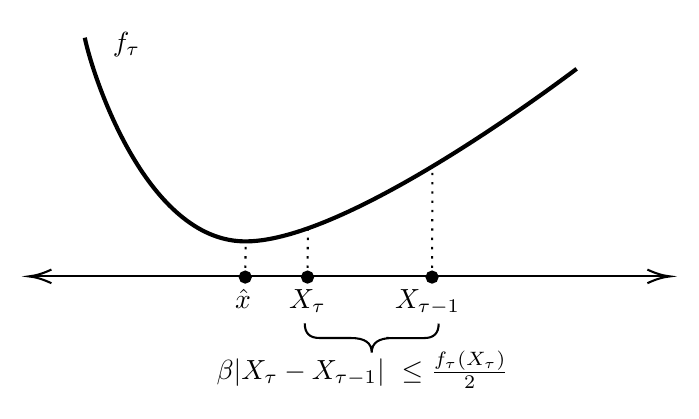
\begin{tikzpicture}[x=0.75pt,y=0.75pt,yscale=-1,xscale=1]
%uncomment if require: \path (0,308); %set diagram left start at 0, and has height of 308

%Curve Lines [id:da37061921880533877]
\draw [line width=1.5]    (98,85.33) .. controls (102.36,105.81) and (127.25,179.72) .. (172,183.33) .. controls (216.75,186.95) and (312.43,117.26) .. (335,100.33) ;
%Straight Lines [id:da8132100594867722]
\draw    (73,200.33) -- (378,200.33) ;
\draw [shift={(380,200.33)}, rotate = 180] [color={rgb, 255:red, 0; green, 0; blue, 0 }  ][line width=0.75]    (10.93,-3.29) .. controls (6.95,-1.4) and (3.31,-0.3) .. (0,0) .. controls (3.31,0.3) and (6.95,1.4) .. (10.93,3.29)   ;
\draw [shift={(71,200.33)}, rotate = 0] [color={rgb, 255:red, 0; green, 0; blue, 0 }  ][line width=0.75]    (10.93,-3.29) .. controls (6.95,-1.4) and (3.31,-0.3) .. (0,0) .. controls (3.31,0.3) and (6.95,1.4) .. (10.93,3.29)   ;
%Shape: Circle [id:dp2801837798690885]
\draw  [fill={rgb, 255:red, 0; green, 0; blue, 0 }  ,fill opacity=1 ] (172.67,200.67) .. controls (172.67,199.19) and (173.86,198) .. (175.33,198) .. controls (176.81,198) and (178,199.19) .. (178,200.67) .. controls (178,202.14) and (176.81,203.33) .. (175.33,203.33) .. controls (173.86,203.33) and (172.67,202.14) .. (172.67,200.67) -- cycle ;
%Shape: Circle [id:dp9237316574850754]
\draw  [fill={rgb, 255:red, 0; green, 0; blue, 0 }  ,fill opacity=1 ] (262.67,200.67) .. controls (262.67,199.19) and (263.86,198) .. (265.33,198) .. controls (266.81,198) and (268,199.19) .. (268,200.67) .. controls (268,202.14) and (266.81,203.33) .. (265.33,203.33) .. controls (263.86,203.33) and (262.67,202.14) .. (262.67,200.67) -- cycle ;
%Shape: Circle [id:dp045787056716331875]
\draw  [fill={rgb, 255:red, 0; green, 0; blue, 0 }  ,fill opacity=1 ] (202.67,200.67) .. controls (202.67,199.19) and (203.86,198) .. (205.33,198) .. controls (206.81,198) and (208,199.19) .. (208,200.67) .. controls (208,202.14) and (206.81,203.33) .. (205.33,203.33) .. controls (203.86,203.33) and (202.67,202.14) .. (202.67,200.67) -- cycle ;
%Straight Lines [id:da9850850655894281]
\draw    [dash pattern={on 0.84pt off 2.51pt}]  (175.33,200.67) -- (175.52,184.05) ;
%Straight Lines [id:da4019047700825191]
\draw    [dash pattern={on 0.84pt off 2.51pt}]  (205.33,200.67) -- (205.52,177.05) ;
%Straight Lines [id:da23167830177054616]
\draw    [dash pattern={on 0.84pt off 2.51pt}]  (265.33,200.67) -- (265.52,147.05) ;
%Shape: Brace [id:dp024365056849508404]
\draw   (204,223) .. controls (204,227.67) and (206.33,230) .. (211,230) -- (226.26,230.02) .. controls (232.93,230.02) and (236.26,232.35) .. (236.25,237.02) .. controls (236.26,232.35) and (239.59,230.02) .. (246.26,230.03)(243.26,230.03) -- (261.52,230.04) .. controls (266.19,230.05) and (268.52,227.72) .. (268.52,223.05) ;

% Text Node
\draw (169,205) node [anchor=north west][inner sep=0.75pt]    {$\hat{x}$};
% Text Node
\draw (195,205) node [anchor=north west][inner sep=0.75pt]    {$X_{\tau }$};
% Text Node
\draw (246,205) node [anchor=north west][inner sep=0.75pt]    {$X_{\tau -1}$};
% Text Node
\draw (160,235) node [anchor=north west][inner sep=0.75pt]    {$\beta |X_{\tau } -X_{\tau -1} |\ \leq \frac{f_{\tau }( X_{\tau })}{2}$};
% Text Node
\draw (110,81) node [anchor=north west][inner sep=0.75pt]    {$f_{\tau }$};


\end{tikzpicture}
